\documentclass{standalone}
\usepackage{tikz}
\usepackage{ctex,siunitx}
\setCJKmainfont{Noto Serif CJK SC}
\usepackage{tkz-euclide}
\usepackage{amsmath,mhchem}
\usetikzlibrary{patterns, calc}
\usetikzlibrary {decorations.pathmorphing, decorations.pathreplacing, decorations.shapes,}
\begin{document}
\small
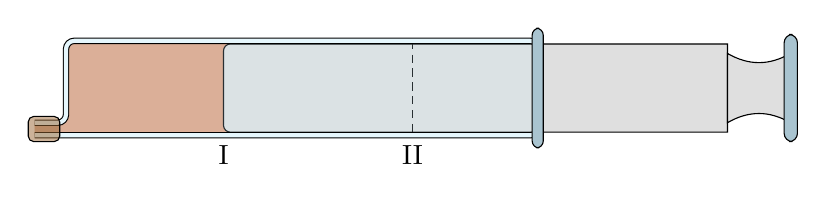
\begin{tikzpicture}[>=stealth,scale=0.8]
  \fill[brown!50!pink](0,0)--(3.2,0)--(3.2,1.5)--(0.5,1.5)--(0.5,0.2)--(0,0.2);
  \draw[fill=lightgray!50!white](3,0.05)--(11,0.05)--(11,1.45)[rounded corners=2.5pt]--(3,1.45)--cycle;
  \draw[densely dashed](6,1.5)--(6,0)node[below]{II};
  \node at (3,0)[below]{I};
  \draw[double=cyan!10!white,double distance=1.5pt,rounded corners=3pt,fill=cyan!20!white,fill opacity=0.2](0,0)--(8,0)--(8,1.5)--(0.5,1.5)--(0.5,0.2)--(0,0.2);
  \draw[rounded corners=2.5pt,fill=cyan!20!lightgray](7.9,-0.2)rectangle++(5pt,1.9);
  \draw[fill=lightgray!50!white](11,1.3)to[bend right](12,1.3)--(12,0.2)to[bend right](11,0.2)--cycle;
  \draw[rounded corners=3pt,fill=cyan!20!lightgray](11.9,-0.1)rectangle++(6pt,1.7);
  \draw[rounded corners=2pt,fill=brown!80!black,fill opacity=0.5](-0.1,-0.1)rectangle(0.4,0.3);
\end{tikzpicture}
\end{document}